\section{Project Management}

\label{sec:projectManagement}

\subsection{Methodology}

The project has been developed incrementally, with a focus on integrating new
functionality completely before progressing to new features. This approach is
well-suited to this project's design: since it consists of five separate areas
which are drawn together at the end, it is possible to focus on implementing a
feature within one area without it affecting the rest. As a result, testing has
been performed throughout and ensures that a newer version of the project is
never worse than its predecessor. Using Git and Github has been helpful in this
regard, providing cloud storage and the ability to roll back to previous
versions of the project if the current one is broken by a new feature.

\begin{figure}[h]
	\centering
	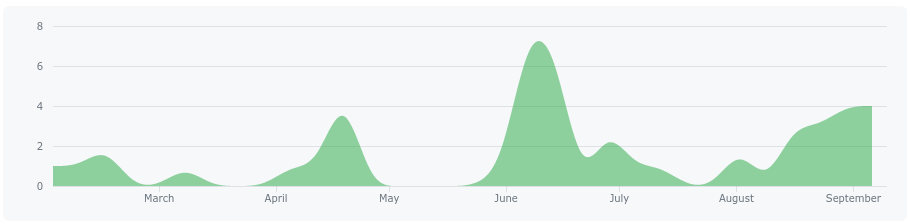
\includegraphics[width=\textwidth]{commits}
	\caption{Commits to Github}
	\label{fig:commits}
\end{figure}

Meetings have been taken with this project's supervisor, Professor Matthias
Englert, to track progress. These were more regular towards the beginning of
the project, though as it began to take shape the consistency of these meetings
declined. As we will discuss in the following section, this is due in part to
the exam period, during which most focus was diverted towards revision, however
the original frequency was never picked up after this time as was initially
planned. Moreover, it bears mentioning that the current situation regarding the
coronavirus pandemic may also have had a part to play in the frequency of these
meetings. Regardless, the author feels more initiative should have been taken
on his end to ensure their consistency, even with the move online.

\subsection{Scheduling}

There have been few major issues with regard to the scheduling of this project,
although it undergone a slight change from the timetable in its original
conception, which was meant to be an implementation of a combinatorial
prediction market similar to \emph{Predictalot}. Figure~\ref{fig:old-timetable}
shows the schedule as it was planned at the time of our presentation on the
project, which was when it was still in its early stages of development. In
Figure~\ref{fig:new-timetable} we detail the order in which tasks were actually
carried out.

\begin{figure}[h]
	\centering
	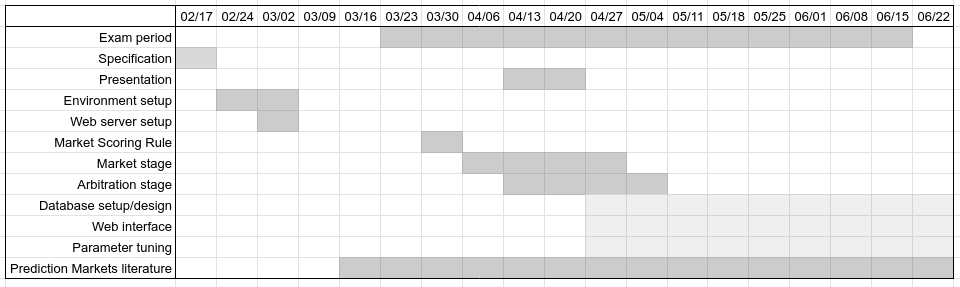
\includegraphics[width=\textwidth]{old-timetable}
	\caption{The project's timetable as it was initially planned}
	\label{fig:old-timetable}
\end{figure}

An initial prototype of the prediction market had been written in time for the
presentation and at its core our current iteration is very similar to this
early version with respect to the datatypes we define and the processes of
trading and arbitration. However, it was entirely text-based and had no
capacity for persistent storage, meaning it was unusable in a practical
setting. At any rate its purpose was to showcase the mechanism in action and
this is, at its core, very simple. 

Work after this point was focused on translating this terminal-based
implementation to operate on a barebones web server, with the first steps to
achieve persistent storage via interaction with a database. Since Mito's
\code{deftable} macro is functionally very similar to that of Common Lisp's
\code{defstruct}, this conversion was relatively straightforward. Similarly,
the code to set up and begin defining webpages in our implementation is simple
and hence took little time. In the case of both the web server and the
database, a significantly larger portion of time was spent deciding how to
integrate features as they were developed into the system as a whole. As we try
to keep our implementation modular there is the implicit requirement to not
only get a feature working in isolation, but to then integrate it into the rest
of the system successfully. This involved constantly updating the web and
database interfaces, and is reflected in Figure~\ref{fig:new-timetable}, which
shows much more overlap between tasks.  Some issues were encountered trying to
implement asynchronous communication with the server via Parenscript and
Smackjack, and much time was spent getting this working. This highlights one of
the drawbacks behind using both libraries: while they are somewhat
well-documented with online reference manuals, it seems they are not widely
used and hence have few practical examples from which to learn.

Worthy of note is the two-week delay from the original deadline for the interim
report, arising from the university-wide implementation of a two-week extension
to all assessed work. We decided to take advantage of this by spending an extra
two weeks to implement the arbitration stage to a greater degree of completion,
in order to have more material for discussion in the interim report. This in
part stems from the fact that we had made less progress during and after the
exam period as expected. This did not affect the overall progress of the
project, however, since the two weeks worth of progress made during this time
was simply borrowed from what would have been achieved in the two weeks after
the original deadline. 

\begin{figure}[h]
	\centering
	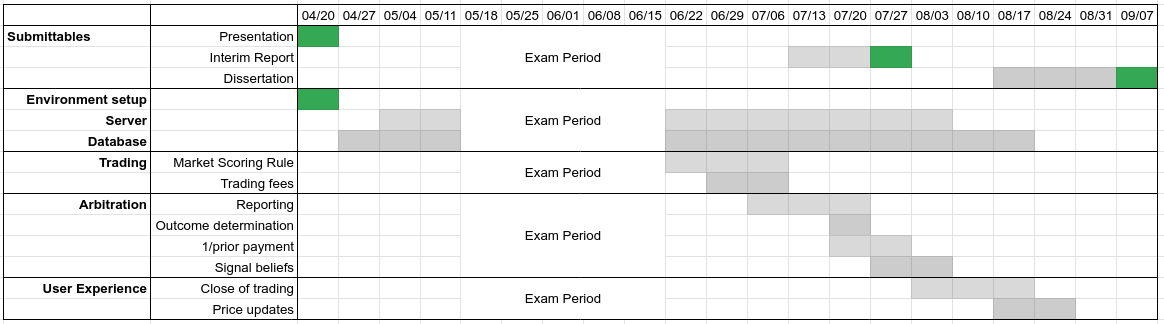
\includegraphics[width=\textwidth]{new-timetable}
	\caption{The realised schedule}
	\label{fig:new-timetable}
\end{figure}

\subsection{Ethics}

There is little ethical consideration required for the development of this
project. All development and testing has been done independently, and all
resources used to implement the system are available freely. Testing has been
performed externally only to small extent, and even then only informally
through gathering opinions amongst colleagues. As we have discussed has been a
problem for existing prediction markets, there is one ethical issue that arises
from using real money in prediction markets and this is their potential to
inspire ``assassination markets'', where there is a real-life incentive to
change the outcome of the market through committing actions of dubious
character, such as assassinating the subject of a security speculating on the
time of their death. We avoid testing the strength of our users' moral fibre by
using fake money only, with no real-world value, meaning there is no incentive
to act in such a way as to compromise one's integrity for monetary gain.
